\documentclass[12pt,a4paper]{article}

\usepackage[utf8]{inputenc}
\usepackage[T1]{fontenc}
\usepackage[english]{babel}
\usepackage{amsmath}
\usepackage{amsfonts}
\usepackage{amssymb}
\usepackage{graphicx}
\usepackage{geometry}
\usepackage{listings}
\usepackage{xcolor}
\usepackage{hyperref}
\usepackage{float}
\usepackage{tikz}
\usetikzlibrary{automata, positioning, arrows.meta}

\geometry{hmargin=2.5cm,vmargin=2.5cm}

\definecolor{codegreen}{rgb}{0,0.6,0}
\definecolor{codegray}{rgb}{0.5,0.5,0.5}
\definecolor{codepurple}{rgb}{0.58,0,0.82}
\definecolor{backcolour}{rgb}{0.95,0.95,0.92}

\lstdefinestyle{vhdlstyle}{
    backgroundcolor=\color{backcolour},
    commentstyle=\color{codegreen},
    keywordstyle=\color{magenta},
    numberstyle=\tiny\color{codegray},
    stringstyle=\color{codepurple},
    basicstyle=\ttfamily\footnotesize,
    breakatwhitespace=false,         
    breaklines=true,                 
    captionpos=b,                    
    keepspaces=true,                 
    numbers=left,                    
    numbersep=5pt,                  
    showspaces=false,                
    showstringspaces=false,
    showtabs=false,                  
    tabsize=2,
    language=VHDL
}

\lstset{style=vhdlstyle}

\title{Project Report - ELEN0040 \\ Whack-a-mole}
\author{Pierre \textbf{SLUSE}, Ilan \textbf{NOMDEFAMILLE}, Gauthier \textbf{NOMDEFAMILLE} }
\date{\today}
\begin{document}

\maketitle


\tableofcontents
\newpage

\section{Introduction}
This project was carried out as part of the Digital Electronics course (ELEN0040). The objective is to design and implement a classic "Whack-a-mole" game on a CPLD (Complex Programmable Logic Device).

The game consists of hitting "moles" represented by LEDs that light up randomly on a grid. The player must press the button corresponding to the lit LED to score points within a limited time. This implementation utilizes fundamental digital logic concepts such as Finite State Machines (FSM), clock synchronization, and pseudo-random number generation via a Linear Feedback Shift Register (LFSR).

\newpage
\section{System Specifications}

\subsection{Game Interface}
The user interface consists of:
\begin{itemize}
    \item \textbf{9 LEDs}: Arranged in a grid, representing the mole locations.
    \item \textbf{9 Buttons}: Each associated with an LED.
    \item \textbf{1 Start Button}: To initiate a new game session.
    \item \textbf{Score Signals}: `score\_high` and `score\_low` to drive an external display or counter.
\end{itemize}

\subsection{Inputs and Outputs Signals}
The following table summarizes the signals of the main \texttt{Whackamole} entity:

\begin{table}[H]
\centering
\begin{tabular}{|l|c|c|l|}
\hline
\textbf{Signal} & \textbf{Pin (MAX V)} & \textbf{Direction} & \textbf{Description} \\ \hline
\texttt{fastclock} & PIN\_7 & Input & Main system clock \\ \hline
\texttt{slowclock} & PIN\_9 & Input & Timer reference clock \\ \hline
\texttt{startButton} & PIN\_21 & Input & Game start initialization \\ \hline
\texttt{button[8:0]} & PIN\_54 to 63 & Input & 9-button grid inputs \\ \hline
\texttt{leds[8:0]} & PIN\_25 to 53 & Output & 9-LED grid outputs \\ \hline
\texttt{score\_high} & PIN\_24 & Output & Success pulse (+1 point) \\ \hline
\texttt{score\_reset} & PIN\_22 & Output & Score reset signal \\ \hline
\end{tabular}
\caption{Pin Assignments on the 5M160ZE64C5 CPLD}
\end{table}

To define this interface in VHDL, the main entity \texttt{Whackamole} is declared as follows:
\begin{lstlisting}[language=VHDL]
entity Whackamole is
  port (
    fastclock   : in  std_logic;
    slowclock   : in  std_logic;
    button      : in  std_logic_vector(8 downto 0);
    startButton : in  std_logic;
    leds        : out std_logic_vector(8 downto 0);
    score_reset : out std_logic;
    score_high  : out std_logic;
    score_low   : out std_logic 
  );
end entity Whackamole;
\end{lstlisting}
\newpage
\section{Logic Architecture}

\subsection{Code Structure}
The logic of the \texttt{Whackamole} entity is implemented as a monolithic sequential process triggered by the rising edge of the \texttt{fastclock}. This design choice means all functionalities (timers, random generation, state management) are evaluated sequentially in one central block:
\begin{lstlisting}[language=VHDL]
main : process(fastclock)
begin
    if rising_edge(fastclock) then
        -- LFSR, Timers, and FSM evaluated here
    end if;
end process;
\end{lstlisting}
We found this approach to be the easiest to implement and the most pertinent for this usage, since the number of states of this machine is quite small, and because almost every event is dependant of a clock, or at least a timer. This allows us to level up or level down the difficulty, depending on the player's preference, using the timers of the CPLD. We needed synchronization of events, and this approach was picked instinctively because it felt like the best approach to synchronize everything together. 

\subsection{Finite State Machine (FSM)}
The core control logic of the game is implemented as a finite state machine with two primary states:
\begin{itemize}
    \item \textbf{IDLE}: The default state upon power-up and game over. In this state, all LEDs blink synchronously with the \texttt{slowclock} to attract attention and indicate readiness. The system transitions to \texttt{PLAY} when the \texttt{startButton} is pressed.
    \item \textbf{PLAY}: The active game state lasting 30 ticks. The logic handles mole generation, hit detection, and score pulsing. When the \texttt{game\_duration\_timer} reaches zero, the system returns to \texttt{IDLE}.
\end{itemize}

\begin{figure}[H]
    \centering
    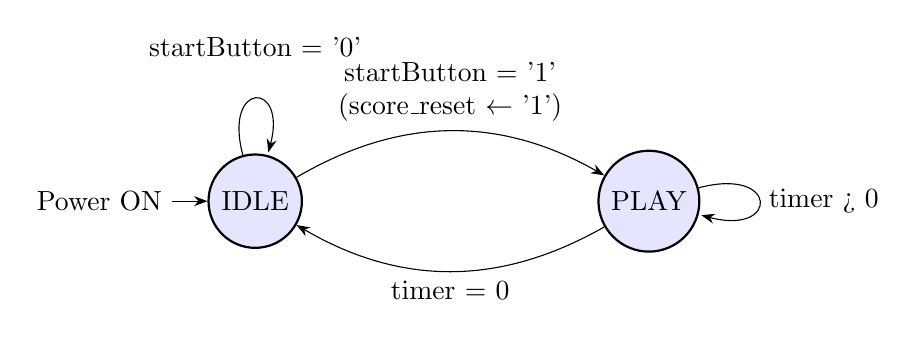
\begin{tikzpicture}[->, >=Stealth, node distance=5cm, every state/.style={thick, fill=blue!10}, initial text={Power ON}]
        \node[state, initial] (IDLE) {IDLE};
        \node[state, right of=IDLE] (PLAY) {PLAY};

        \path (IDLE) edge [loop above] node [align=center] {startButton = '0'\\} (IDLE)
              (IDLE) edge [bend left] node [above, align=center] {startButton = '1' \\ (score\_reset $\gets$ '1')} (PLAY)
              (PLAY) edge [loop right] node [align=center] {timer > 0} (PLAY)
              (PLAY) edge [bend left] node [below, align=center] {timer = 0} (IDLE);
    \end{tikzpicture}
    \caption{representation of the Finite State Machine}
\end{figure}

The initialization and transition of these states are managed within the main process. We defined a custom \texttt{state\_type} to handle the logic cleanly:
\begin{lstlisting}[language=VHDL]
type state_type is (IDLE, PLAY);
signal state : state_type := IDLE;
-- ... inside the main process
case state is
    when IDLE =>
        -- LEDs blink with slowclock, wait for start
        leds <= (others => slowclock);
        if startButton = '1' and start_pressed = '0' then
            state <= PLAY;
            game_duration_timer <= 30;
        end if;
    when PLAY =>
        -- Main game logic
        -- Game ends when timer reaches 0
        if game_duration_timer = 0 then
            state <= IDLE;
        end if;
end case;
\end{lstlisting}

\subsection{Pseudo-Random Generation (LFSR)}
To ensure the unpredictability of mole appearances, we searched the Internet to find a suitable random number generation method, and instead of picking up the output of an unpredictable entry (ex : floating input gate or 555 timer running a 4 bit shift register very fast), we found that we could implement an LFSR, Linear-Feedback shift register. Thus we implemented a 5-bit LFSR is implemented. This component generates a sequence of numbers that appears random despite being deterministic. The polynomial used is $x^5 + x^3 + 1$. 
\begin{lstlisting}[language=VHDL]
-- LFSR update code snippet
lfsr <= lfsr(3 downto 0) & (lfsr(4) xor lfsr(2));
\end{lstlisting}
At each \texttt{fastclock} cycle, the register evolves. When the system decides to spawn a new mole, the current value of the LFSR (truncated to 4 bits) is converted to an index between 0 and 8, used to light up one of the nine output LEDs. The sequence begins with [1 0 0 0 0] to ensure that the pattern does not start repeating itself (ex : [ 0 0 0 0 0 ] would repeat zeros indefinitely, we tried. Since we do not know when the user will start the game, when the user is waiting in the \textbf{IDLE} state, the fastclock has plenty of time to run and "randomize" this LFSR. 

\subsection{Time Management and Synchronization}
The system uses two clocks passed through the ports:
\begin{itemize}
    \item \texttt{fastclock}: Used for fast sequential logic (LFSR, edge detection).
    \item \texttt{slowclock}: Used as a time reference for the game countdown and for flashing LEDs in IDLE mode. Since we don't count time as "seconds" but rather as ticks, we can then adjust the slow clock to adapt the length of the game, thus the difficulty. 
\end{itemize}
An internal \texttt{global\_tick} counter (0 to 63) acts as a pre-divider to pace the appearance of moles and their duration on the screen. This approach is more efficient than individual per-mole counters, since it does use fewer timers, and thus precious logic cells. 

Here is how the timer updates are implemented in VHDL. We use a \texttt{slowclock\_prev} signal to detect the rising edge of the slow clock synchronously within the \texttt{fastclock} process:
\begin{lstlisting}[language=VHDL]
-- Total game timer management using slowclock edge detection
if slowclock = '1' and slowclock_prev = '0' then
    if game_duration_timer > 0 then
        game_duration_timer <= game_duration_timer - 1;
    else
        state <= IDLE;
    end if;
end if;

-- Global Tick Prescaler (0 to 63) based on fastclock
if global_tick = 63 then
    global_tick <= 0;
else
    global_tick <= global_tick + 1;
end if;
\end{lstlisting}

\subsection{Game Logic and Hit Detection}
During the \texttt{PLAY} state, the system continuously iterates over the 9 buttons to detect rising edges (button presses). We use a strictly synchronous hit detection mechanism:
\begin{lstlisting}[language=VHDL]
-- Edge detection for independent hit detection
if button(i) = '1' and button_pressed(i) = '0' then
    if mole_active(i) = '1' then
        score_timer <= 31;      -- Trigger success pulse
        mole_active(i) <= '0';  -- Deactivate mole
    else
        wrong_click := true;    -- Flag for penalty
    end if;
end if;
\end{lstlisting}
\begin{itemize}
    \item \textbf{Spawning}: A new mole appears if the number of active moles is less than 2.
    \item \textbf{Hit}: Successfully hitting an active mole activates the \texttt{score\_high} signal for 31 clock cycles. (long enough for the 4026B chip to register an input)   
    \item \textbf{Miss/Error}: If an error is flagged (\texttt{wrong\_click}), the \texttt{score\_low} signal is activated and a 1-tick penalty is applied to the remaining game time.
\end{itemize}

\newpage
\section{Hardware Validation}
Unlike traditional workflows relying on functional VHDL simulations or testbenches, the validation of this project was performed entirely live on real hardware. 

The VHDL code was continuously synthesized and programmed onto the MAX V CPLD via Quartus. The physical interfacing via the real buttons and LEDs allowed for immediate, tactile testing of critical edge cases:
\begin{itemize}
    \item Verifying that rapid consecutive button presses register properly.
    \item Confirming the exact visual duration of the moles and LED feedback on the breadboard.
    \item Ensuring the penalty timer strictly reduces the overall game time upon erroneous inputs.
\end{itemize}
This hands-on approach ensured the system's robustness under physical constraints and eliminated the need for abstract software simulation. Since we could afford to build a prototype rightaway, we used this prototype to iterate a lot more quickly than editing our test bench and seeing our program fail miserably in real conditions. We are aware that this approach is not the best one, since building a prototype before designing the logic circuit can become very expensive pretty quickly, and that in many cases it is not possible to do, however the project was small enough to let us build the circuit in parallel of programming the CPLD

\newpage
\section{Hardware Implementation}
The design was optimized to minimize logic element usage while maintaining a clear state separation. We chose to use the CPLD in combination with CD4026B chips to display the score, to not overwhelm the CPLD with unnessecary  data (remembering the pattern for each number on an 8 segment display), simplyfy the code and also try to use the CPLD not just as the whole circuit but to be integrated more as a brain in a more complex circuit. 
We used a tool called KiCAD to design the schematic of the circuit, using real component references, and a schematic of the CPLD development board. 

\begin{figure}[H] % [H] pour forcer la position ici
    \centering
    % On utilise \includegraphics pour le PDF. 
    % 'page=1' insère la première page. 
    % 'width' ajuste la taille à la largeur du texte.
    \includegraphics[width=1\linewidth, page=1]{Circuit-schematic.pdf}
    \caption{Electronic schematic of the system (KiCAD)}
    \label{fig:schematic}
\end{figure}
The schematic shows clearly debouncing circuits on each of the buttons, to ensure that every click is only registered once, and does not need to be filtered digitally. On the final design those circuits are barely visible, and it's for a simple reason : We used  0804 and 0402 SMD components (resistors and capacitors) to build the debouncing circuits, to take less space first, but also because those components are a lot less expensive to get in bulk. 


\begin{figure}
    \centering
    \includegraphics[width=1\linewidth]{compilation_report.png}
    \caption{Screenshot of the compilation report and resources usage}
    \label{fig:placeholder}
\end{figure}
\newpage
\section{Conclusion}
The "Whack-a-mole" project allowed us to apply synchronization concepts for asynchronous events (buttons) and real-time management on a CPLD. The use of an LFSR added an interesting layer of complexity to randomness management, while the FSM structured the global behavior robustly. 



\end{document}
